
La dernière alerte modélisée est le cas dit du \enquote{fil rouge} que
nous avions présenté dans le premier chapitre de cette thèse. Comme
nous l'avions indiqué lors de sa première présentation, le \emph{fil
  rouge} est une alerte particulière, contenant de nombreux indices
très imprécis et incertains. Par conséquent la \ac{zir} est
extrêmement étendue.


\subsection{Présentation de l'alerte}
\label{subsec:9-4-1}

Le fil rouge est une alerte composée de XX \emph{indices de
  localisation.}




Faute d'enregistrement audio, le fil rouge n'a pas été retranscrit,
les indices dont nous disposons (et qui avaient été présentés dans le
\autoref{chap:01}) ont donc été directement saisis par le secouriste.
%
de ce fait, le \emph{fil rouge} est une alerte assez différente des
précédentes, puisque XXX n'est pas
%
Le traitement du \emph{fil rouge} est donc plus proche du traitement
opérationnel qui sera réellement effectué lors du traitement d'une
alerte.



\begin{figure}
  \centering
  \begin{tikzpicture}
  \tikzset{et/.style={above,font=\footnotesize\vphantom{Ag}}}
  % 
  \node[inner sep=0pt, anchor=south west] (image) at (0,0){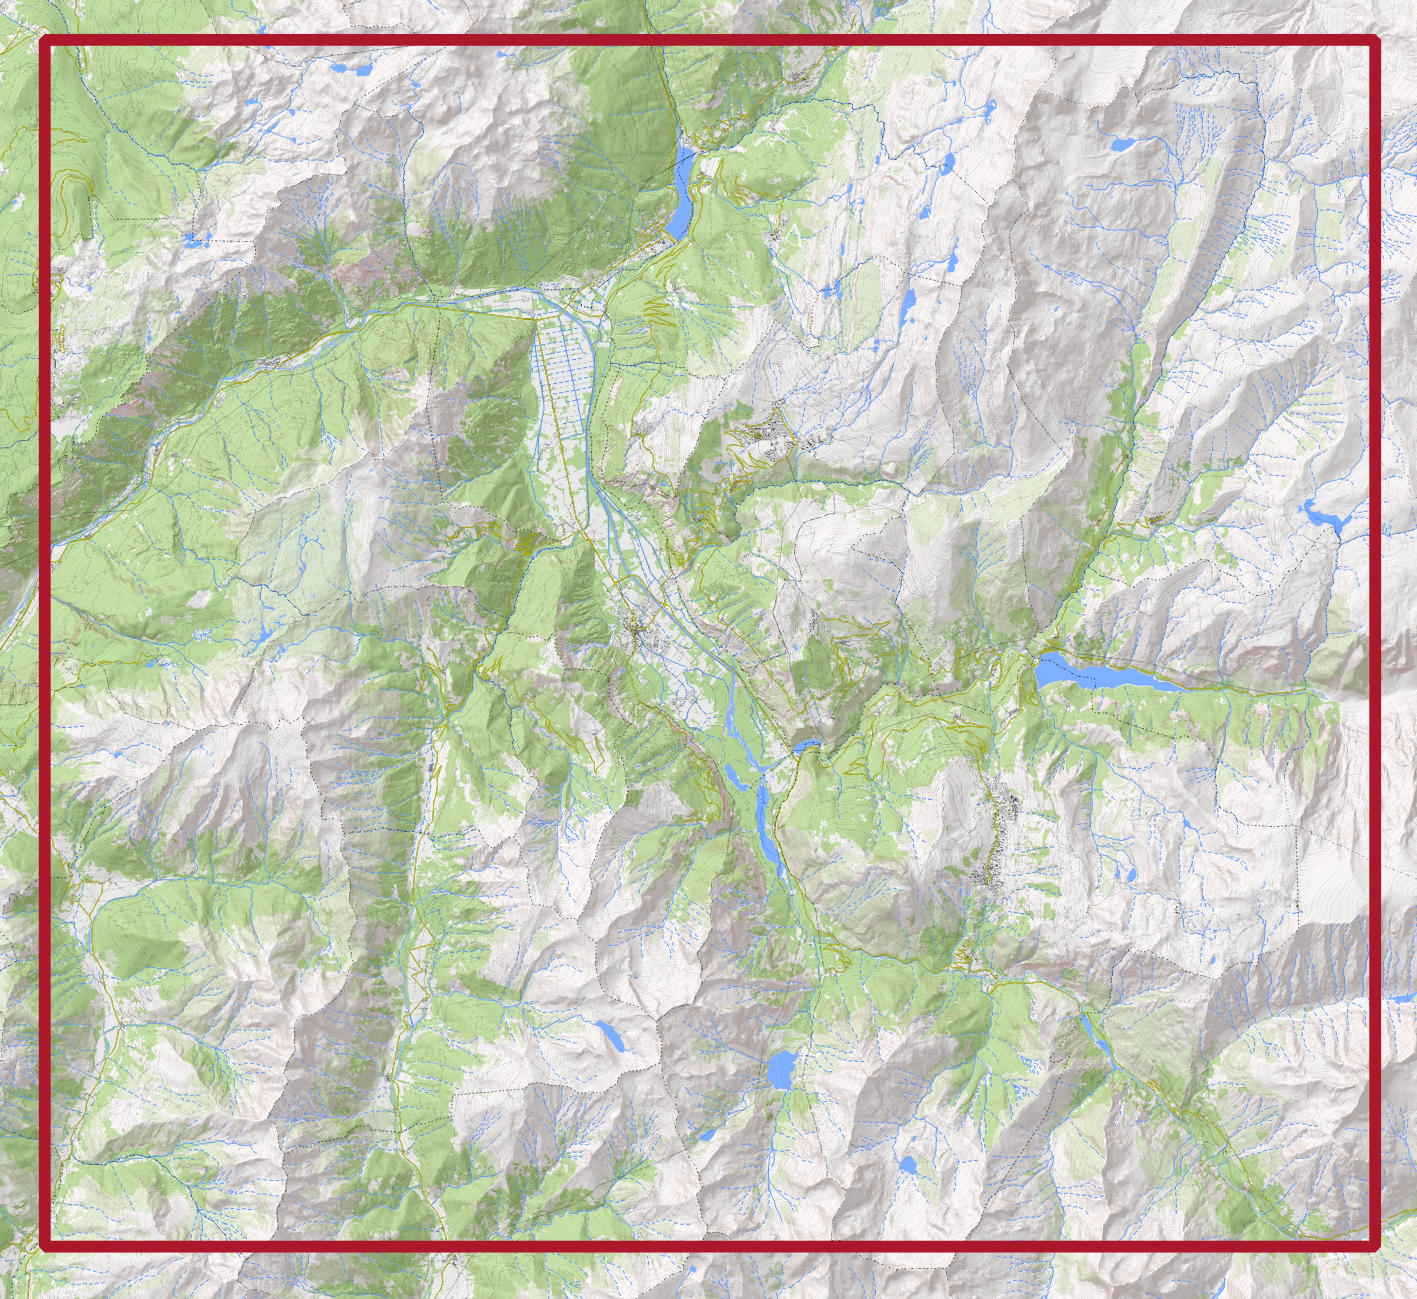
\includegraphics{./figures/ZIR_fil_rouge.png}};
  % 
  \begin{scope}
    \node (P2) at ([yshift=-.5cm]image.south east) {};
    \node (P1) at ([yshift=-.5cm]image.south west) {};
    % 
    \node (rect) [anchor=north west, minimum width=1cm,minimum
    height=.25cm] at ([yshift=-.25cm]P1) {}; \path[draw=RdBu-9-1, line
    width=1mm](rect.west) --([xshift=-1ex]rect.south) -- ([xshift=1ex]rect.north)
    -- (rect.east);
    % 
    \node[anchor=west, font=\tiny\vphantom{Ag}, text width = 4cm] at
    ([xshift=1ex]rect.east) {Limite de la \ac{zir}};
    % Échelle
    % Échelle
    \draw[-] (P2 |- -1cm,-1cm) --++ (-1,0) node[et,pos=.5] {\SI{2}{\kilo\meter}};
    % Légende détaillée
    \path (P1) -- (P2) node[pos=.5, yshift=-1cm] {\tiny Pour la légende détaillée du fond topographique voir \autoref{anx:topo_leg}. Sources: BD TOPO 2018, BD ALTI 2018.}; 
  \end{scope}
\end{tikzpicture}
  \caption{Zone initiale de recherche pour le \emph{fil rouge}}
  \label{fig:zir_fil_rouge}
\end{figure}

Pour le cas du \emph{fil rouge} nous ne disposons pas de
l'enregistrement audio et donc de son verbatim, les indices ayant déjà 
été synthétisés par les secouristes. Les les avions déjà présentés
dans le \autoref{chap:01}.
%
Pour rappel voici la synthèse de l'alerte qui nous a été donnée par
les secouristes :
%
\begin{enumerate}
\item La victime est partie de \emph{Bourg-d'Oisans,} à pied, sur
  chemin, en direction d'une station de ski.
\item La victime a marché plusieurs heures.
\item La victime a chuté de plusieurs mètres.
\item La victime voit une partie de plan d'eau.
\item La victime est sous une route et entend des véhicules.
\item La victime est sous une ligne électrique 3 brins.
\item La victime vient de passer du soleil à l'ombre.
\item Le téléphone de la victime est connecté à une antenne GSM située
  à la chapelle \emph{St-Philomene} à \emph{Villard-Reymond} et
  orientée à \SI{90}{\degree}
\end{enumerate}

Comme nous l'avions déjà signalé lors de la présentation du \emph{fil
  rouge} (\autoref{chap:01}), ces différentes informations sont
fortement imprécises, surtout si on les compare aux extraits des
alertes \emph{Grand Veymont} (\autoref{anx:retrans_grand_veymont}) et
\emph{Moucherotte} (\autoref{anx:retrans_moucherotte}). Les
descriptions sont ici peu informatives et discriminantes et la
construction d'indices de localisations est par conséquent plus
délicate.

La première de ces sept descriptions donne plusieurs informations sur
le trajet suivit par la victime jusqu'à sa position actuelle. Elle
nous renseigne sur son point de départ, clairement identifié, sa
destination visée, une station de ski inconnue et son mode de
déplacement, à pied sur un chemin. Ces informations ne sont cependant
pas directement transposables en un indice de localisation. On
pourrait certes supposer qu'étant donné que \enquote{La victime est
  partie de \emph{Bourg-d'Oisans}}, elle est probablement à proximité
de cette ville, ce qui permettrait d'utiliser les relations de
localisations \onto[orl]{Aux\-Alentours\-De} ou
\onto[orl]{Proximal}. Cependant, rien dans cette première description
ne nous permet d'affirmer que la victime est toujours à proximité de
\emph{Bourg-d'Oisans.} En effet, nous ne connaissons pas la durée de
sa sortie et il se peut que la victime ait parcouru suffisamment de
kilomètres pour que ces relations de localisaiton ne soient plus
valides. Il nous semble donc prématuré d'utiliser ces relations de
localisaiton. De manière similaire nous pourrions envisager d'utiliser
la relation de localisation
\onto[orla]{Si\-tue\-Sur\-Itineraire\-Ou\-Reseau\-Support}, la victime
ayant indiqué avoir utilisé un chemin. Cependant, les expressions
suivantes nous indiquent que la victime \enquote{a chuté de plusieurs
  mètres}. Il est par conséquent difficile d'affirmer que la victime
se situe toujours sur un chemin, c'est pourquoi il ne nous semble pas
pertinent d'utiliser cette relation de localisaiton. Il est cependant
possible de construire un indice de localisation à partir de cette
première description. En effet, la victime indique qu'elle est partie
de \emph{Bourg-d'Oisans} dans la direction \enquote{globale} d'une
station de ski, ce qui nous renseigne sur sa direction globale. Or, la
relation de localisation
\onto[orl]{Dans\-La\-Direction\-De\-X\-Depuis\-Y} a été conçue pour
modéliser ce type d'informations, sans préjuger du mode ou du support
de déplacement.

Le second élément de cette alerte, \enquote{La victime a marché
  plusieurs heures}, donne un premier complément d'informations aux
informations précédentes. Grâce à la connaissance du point de départ
et à l'identification du temps de déplacement, nous pouvons construire
une estimation de la distance parcourue par la victime. Pour ce faire
nous avons défini une relation de localisation
\onto[orl]{A\-Temps\-De\-Marche\-De}, permettant de construire la
\ac{zlc} atteignable en un temps de marche et à partir d'un point de
départ donné. La possibilité de construire un tel indice de
localisation remplace avantageusement l'utilisation d'une relation de
localisation telle que \onto[orl]{Aux\-Alentours\-De}. En effet, cette
dernière ne donne qu'une information très vague sur la zone de
présence de la victime, alors que la relation de localisation
\onto[orl]{A\-Temps\-De\-Marche\-De} permet une modélisation plus
fine, même dans le cas présent, où l'estimation du temps de parcours
est très imprécise. Dans le cas de cette alerte nous avons donc
considéré qu'il était inutile de définir un indice de localisation
employant les relations de localisaiton \onto[orl]{Aux\-Alentours\-De}
ou \onto[orl]{Proximal}, la relation
\onto[orl]{A\-Temps\-De\-Marche\-De} quantifiant également un
éloignement au point de départ, mais de manière plus discriminante.

Le troisième élément de l'alerte nous indique que \enquote{la victime
  a chuté de plusieurs mètres}. Prise sous cette forme, cette
description n'est pas interprétable comme un indice de localisation et
aucune des relations que nous avons définies ne permet de
l'exprimer. Il est cependant possible de combiner cette information
avec les descriptions précédentes, de manière à construire un nouvel
indice de localisation. Ces descriptions nous renseignent, en effet,
sur le potentiel contexte de cette chute. Comme la victime a indiqué
qu'elle se déplaçait à pied, sur un chemin, nous pouvons supposer que
c'était également le cas lors de sa chute. Nous pouvons alors en
déduire que, suite à sa chute, la victime se situe sous un
chemin. Cette information extrapolée peut ainsi être modélisée avec la
relation de localisation \onto[orl]{Sous\-Altitude} ou l'une des
relations qui en dérivent. Compte-tenu du contexte de la chute, la
relation de localisation plus appropriée nous semble être
\onto[orl]{Sous\-Proche\-De}, puisqu’elle ajoute une contrainte de
proximité planimétrique. Ainsi s'il nous est impossible de construire
directement une \ac{zlc} grâce à l'information \enquote{J'ai chuté de
  plusieurs mètres}, il nous est en revanche possible de dériver de
cette information un indice de localisation exprimant la position
actuelle de la victime, par rapport au chemin dont elle vient de
chuter.

L'interprétation de la quatrième description de l'alerte, \enquote{La
  victime voit une partie d'un plan d'eau}, est plus évidente que
celle des descriptions précédentes. En effet, deux relations de
localisation spécifiques ont été introduites pour traiter des
relations de visibilité \onto[orl]{Site\-Voit\-Cible} et
\onto[orl]{Cible\-Voit\-Site}. Ces différentes relations permettent de
distinguer les visibilités actives et passives. Dans le cas présent,
la victime décrit ce qu'elle voit, on est donc dans une situation
modélisable à l'aide de la relation de localisation
\onto[orl]{Cible\-Voit\-Site}. Cette description présente cependant la
particularité d'employer l’adverbe \enquote{presque} précisant que le
plan d'eau mentionné n'est pas vu dans son intégralité. Dans sa
configuration initiale la relation \onto[orl]{Cible\-Voit\-Site} ne
permet pas d'exprimer une telle description, il est donc nécessaire
d'employer un modifieur, ce que nous détaillerons lors de la
modélisation de cet indice de localisation.

De manière similaire, la cinquième description, \enquote{La victime
  est sous une route et entend des voitures}, est assez explicite. On
reconnait dans cette formulation l'utilisation de la préposition
\enquote{sous} traduisant une relation de verticalité. Or, comme nous
l'indiquions lors de l'analyse de la seconde description (\enquote{La
  victime a chuté de plusieurs mètres}), la relation de localisation
\onto{Sous\-Altitude}, n'apportant aucune contrainte sur l'axe
horizontal, n'est pas nécessairement la plus pertinente ici. On peut
donc utiliser une nouvelle fois la relation de localisation
\onto[orl]{Sous\-Proche\-De} pour construire un nouvel indice de
localisation. Cette description donne une seconde information,
\enquote{la victime entend des véhicules}. Cette dernière n'est, une
nouvelle, pas directement interprétable avec une relation de
localisation, pourtant cette information peut être exploitée de
manière à raffiner la modélisation de \emph{l'indice de localisation.}
On peut tirer deux informations différentes de cette indication. Tout
d'abord une indication de proximité. En effet, la victime indique
indirectement qu'elle se situe a portée de son de la route, ce qui, si
l'on disposait d'un modèle adapté, permettrait d'estimer la distance
de victime à la route.Il serait même possible de définir une nouvelle
relation de localisation \onto{A\-Porte\-De\-Son} pour retranscrire
cette indication. Une telle relation permettrait sans aucun doute
d'affiner cette approximation, particulièrement si elle permet la
prise en compte des effets d’échos, particulièrement présents en
montagne, pouvant conduire à une perception faussée de la distance
d'un son. Cependant nous n'avons pas travaillé au développement d'une
telle méthode, cette alerte étant la seule où une portée sonore est
mentionnée. La seconde information que l'on peut tirer de cet élément
est la nature de la route. On peut en effet considérer que, pour que
la victime note entendre une route, il est nécessaire que celle-ci
soit suffisamment fréquentée pour que le trafic soit notable. Un tel
critère permet d'affiner la sélection des objets de référence, qui,
compte-tenu de l’imprécision de la description, seront relativement
nombreux. Il est cependant délicat de procéder à une telle sélection
sans risquer de supprimer des objets de référence pertinents, et donc
de créer des faux négatifs. En effet, l'hypothèse que nous proposons
ici est assez contraignante et il nous semble inenvisageable de
l'appliquer sans la confirmation de la victime.

Dans la sixième description, la victime indique qu'elle se situe sous
une ligne électrique trois brins. Nous avons déjà présenté ce cas,
notamment dans le \autoref{chap:06} où nous comparions les différentes
implémentations de la théorie des sous-ensembles flous pour
représenter des zones de localisation. Si nous n'avions pas encore
présenté les différentes relations de localisation, définies dans
l'ontologie des relations de localisation, nous avions déjà expliqué
que cette description nécessitait que la relation de verticalité entre
le \emph{site} et la \emph{cible} soit contrainte selon l'axe
horizontal. Dit autrement, il est ici nécessaire d'être proche du
\emph{site} et à une altitude inférieure du \emph{site} pour que l'on
puisse affirmer qu'une position soit \enquote{sous} le \emph{site.}
La relation de localisation \onto{Sous\-Proche\-De} a spécifiquement
été définie pour modéliser ce type de relation.

La septième description donnée par le secouriste nous indique que la
position de la victime vient de passer du Soleil à l'ombre. Une
nouvelle fois nous n'avons pas défini de relation de localisation
permettant de modéliser un tel indice, celui-ci n'apparaissant qu'une
seule fois dans l'ensemble du corpus d'alertes. Il serait cependant
possible de mettre en place une telle relation de localisation,
plusieurs bibliothèques permettant de modéliser les ombres produites
par le relief en fonction de l'heure de la journée.

La huitième et dernière information que nous ayons sur cette alerte
donne la position du relais téléphonique auquel le téléphone de la
victime est connecté. Comme pour la description précédente nous
n'avons pas défini une relation de localisation spécifique à ce type
d'information, mais pour des raisons différentes. En effet, si
l’indication \enquote{Je viens de passer du Soleil à l'ombre} est
unique, ce qui nous a conduit à l'ignorer provisoirement, la
connaissance de l'antenne de rattachement du téléphone de la victime
est plus fréquente. Toutefois l'exploitation fine de cet indice est
assez complexe, comme nous l'avions rapidement évoqué dans le
\autoref{chap:01}. L'implémentation d'une hypothétique relation
\onto{Connecte\-A\-Antenne} nécessiterai, en effet, de prendre la
portée du signal, fortement influencée par les conditions
climatiques. Nous avons donc choisi d'ajourner sa définition. Il est
cependant possible d'utiliser cette information pour extrapoler un
nouvel indice de localisation, certes moins précis que celui que l'on
pourrait obtenir avec une relation de localisation dédiée, mais tout
de même discriminant. On connait en effet l'orientation générale de
l'antenne téléphonique de à laquelle le téléphone de la victime est
connecté. On peut alors approximer la zone où le téléphone de la
victime peut se connecter à une antenne donnée en l'approximant à
l'aide d'une relation cardinale. On peut ici employer la relation de
localisation \onto[orl]{A\-L\-Est\-De}, pour créer ce cône. Il n'y a
ici pas de raisons d'employer une des relations de localisation
dérivée de \onto[orl]{A\-L\-Est\-De}, comme
\onto[orl]{Dans\-La\-Partie\-Est\-De} ou
\onto[orl]{A\-L\-Est\-De\-Externe}. En effet, l'objet de référence
utilisé pour cet indice de localisation, une antenne GSM, n'est pas de
taille suffisante pour que cette distinction est un sens. Cette
approche ne permettra cependant pas de modéliser la portée du signal,
le cône construit par la relation \onto[orl]{A\-L\-Est\-De} étant
virtuellement infini. Cette approximation dans la modélisation de ce
dernier indice est certes insatisfaisante en soi, mais elle devient
parfaitement acceptable lorsque remise dans le contexte de la
modélisation de l'alerte dans son ensemble, la multiplication des
indices de localisation permettant de compenser la faiblesse de
certains d'entre eux.

Au terme de l'analyse de l'alerte on dispose donc de 7 indices de
localisation à spatialiser:
% 
\begin{enumerate}
\item \label{ind:fr1} La victime est
  \onto[orl]{Dans\-La\-Direction\-De\-X\-Depuis\-Y}
  \emph{Bourg-d'Oisans} (\texttt{X}) et une station de ski
  (\texttt{Y})
  % 
\item \label{ind:fr2} La victime est
  \onto[orl]{A\-Temps\-De\-Marche\-De} \emph{Bourg-d'Oisans} 
  % 
\item \label{ind:fr3} La victime est \onto[orl]{Sous\-Proche\-De} un
  chemin
  % 
\item \label{ind:fr4} La victime voit (\onto[orl]{Cible\-Voit\-Site})
  une partie d'un plan d'eau
  % 
\item \label{ind:fr5} La victime est \onto[orl]{Sous\-Proche\-De} une
  route
  % 
\item \label{ind:fr6} La victime est \onto[orl]{Sous\-Proche\-De} une
  ligne électrique trois brins
  % 
\item \label{ind:fr7} La victime est \onto[orl]{A\-L\-Est\-De}
  l'antenne GSM de la \emph{St-Philomene}
\end{enumerate}

\subsection{Modélisation de l'alerte}
\label{subsec:9-4-2}

Les informations données par la victime étant très imprécises, il est
difficile de définir la \emph{zone initiale de recherche} pour cette
alerte. On sait cependant, grâce au premier indice de localisation
(\ref{ind:fr1}), que la victime est partie de Bourg-d'Oisans, on peut
donc centrer la \ac{zir} sur ce lieu. Cependant, aucun autre indice de
nous permet d'estimer la taille que devrait faire cette zone. Nous
avons donc pris la décision de définir une \ac{zir} dont les limites
ne seraient pas atteignables en une journée par un randonneur (à moins
qu'il se déplace en fond de vallée).
%
Nous avons donc créé une \ac{zir} de \SI{25}{\kilo\meter} de côté,
pour une aire de \SI{625}{\kilo\meter\squared}
(\autoref{fig:zir_fil_rouge}).

% Direction
Le premier des indices de localisation de cette alerte (\ref{ind:fr1})
est fondé sur la relation de localisation
\onto[orl]{Dans\-La\-Direction\-De\-X\-Depuis\-Y}, qui permet de
modéliser une relation de direction sans considération d'itinéraire ou
de support. Il s'agit d'une relation de localisation atomique
utilisant le rasteriser \onto[orla]{Centroide}, la métrique
\onto[orla]{XXX} et le fuzzyficateur \onto[orla]{XXXX}
(\autoref{fig:ex_parties_statialisation_DanslaDirectionDe}). Cette
relation de localisation a la particularité d'être binaire, elle
nécessite donc deux sites, \texttt{X} et \texttt{Y}, le premier
donnant le point visé et le second le point de départ. Dans le cas
présent l'un des deux sites est clairement identifié
(\enquote{Bourg-d'Oisans}) alors que le second est désigné par son
type (\enquote{Une station de ski}). Il est donc nécessaire de
procéder à la décomposition de l'indice de localisation en fonction
des différentes instances correspondant à la description de l'objet de
référence. Dans le cas présent on peut identifier 7 stations de ski
\footnote{Les deux Alpes, Auris en Oisans, Ornon, l'Alpe d'Huez, Oz,
  Villard-Reculas et Vaujany.}  dans la \ac{zir}, chacune entre elles
pouvant être un objet de référence potentiel. Nous aurions pu
compléter cette sélection en y ajoutant les stations situées en
bordure de la \ac{zir}, comme \emph{Champrousse,} le requérant pouvant
se diriger vers une station (ce qui justifiait de la sélectionner),
sans qu'il n'ait eut le temps de l'atteindre (ce qui justifie son
absence de la \ac{zir}). Nous avons cependant choisi de nous limiter à
sélectionner les stations situées dans la \ac{zir}, cette dernière
étant de grande taille et une station comme \emph{Champrousse} nous
semblant être trop éloignées du point de départ pour être pertinente.
On est donc amenés à décomposer cet indice de localisation en 7
sous-indices, partageant la même relation de localisation et le même
site \texttt{Y} (\ie le même point de départ) et se distinguant par
leur destination, site \texttt{X}.

\begin{figure}
  \centering
  \input{./figures/exemple_parties_spatialisation_DansLaDirectionDe.tex}
  \caption{Rasteriser, métrique et fuzzyficateur utilisés pour la
    spatialisation de la relation de localisation atomique
    \protect\onto[orla]{Dans\-La\-Direction\-De\-X\-Depuis\-Y}}
  \label{fig:ex_parties_statialisation_DanslaDirectionDe}
\end{figure}

Pour représenter les objets utilisés comme site nous avons, à nouveau,
utilisé les données ponctuelles, destinées au placement des toponymes,
présents dans la BDTOPO. Les géotypes désignés par la victime sont
donc représentés par des points, ce qui est une approximation
significative. Cependant, nous avons choisi d'utiliser le rasteriser
\onto[orla]{Centroide} pour la spatialisation de la relation de
localisation \onto[orl]{Dans\-La\-Direction\-De\-X\-Depuis\-Y},
l'utilisation d'une autre géométrie n'aurait donc pas impacté le
résultat de la modélisation.

Une fois la décomposition effectuée on peut procéder à la
spatialisation indépendante des indices de localisation. L'opération
de rasterisation ne présente pas caractéristiques particulières, si ce
n'est que nous avons choisi d'employer la rasteriser
\onto[orla]{Centroide}, celui-ci nous semblant plus adapté à la
modélisation d'une direction.

Une fois la rasterisation effectuée la métrique
\onto[orla]{Direction\-De} est calculée. Cette métrique, déjà
présentée dans le \autoref{chap:07}, mesure la distance de chaque
position de la \ac{zir} à une ellipse alignée sur la droite reliant
les centroïdes des sites \texttt{X} et \texttt{Y} et dont la taille
(\ie la taille des demi-grand et petit axes) est proportionnelle à la
distance entre \texttt{X} et \texttt{Y}. La figure
\ref{fig:Metrique_FilRouge_1_obj_1} représente le résultat de la
métrique pour l'indice de localisation décomposé : \enquote{La victime
  est partie de \emph{Bourg-d'Oisans} en direction des
  \emph{Deux-Alpes}}. Comme on peut le voir sur cette figure, les deux
sites sont légèrement en dehors de l'ellipse. Nous avons en effet
considéré que cette relation de localisation perdait en pertinence à
proximité des deux sites. Ainsi, nous avons fixé la longueur de
l'ellipse à 90 \% de la longueur du segment reliant les deux sites. La
longueur du demi-grand axe de l'ellipse est quant à elle définie en
fonction de la longueur du demi grand-axe \footnote{Précisément 25 \%
  de la longueur du demi grand-axe.}. En choisissant de faire des deux
axes de l'ellipse des longueurs proportionnelles à la distance
séparant les deux sites de la relation de localisation, nous faisions
l'hypothèse que plus la destination est éloignée de l'origine du
déplacement, plus il est probable que la victime suive un chemin
s'éloignant considérablement de la droite.

Une fois que la métrique a été calculée nous pouvons passer à la
construction de la \ac{zlc} par le biais de la fuzzyfication. La
figure \ref{fig:ZLC_FilRouge_1_obj_1} représente le résultat de la
fuzzyfication de la figure \ref{fig:Metrique_FilRouge_1_obj_1}
\footnote{On pourra remarquer que l'ellipse représentée sur les
  figures \ref{fig:Metrique_FilRouge_1_obj_1} et
  \ref{fig:ZLC_FilRouge_1_obj_1} ne semble pas être parfaitement
  parallèle au segment reliant \emph{Bourg-d'Oisans} aux
  \emph{Deux-Alpes.} Cette déformation est liée au changement de
  résolution effectué pour la représentation de ces résultats et n'est
  donc pas présente à la résolution native.}.
%
La fonction de fuzzyfication choisie, \onto[orla]{Inf\-Val\-0}, a été
paramétrée avec une valeur \(\delta\) de XX.
%
Comme on peut le remarquer, la zone de localisation ainsi construite
inclut et dépasse de part et d'autre des deux sites, même si le degré
d'appartenance est plus faible que celui au centre de l'ellipse. Nous
avons souhaité ce comportement pour prendre en compte d'éventuels
dépassements, potentiellement fréquents en montagne. Ainsi, si la
victime, partant de Bourg-d'Oisans à destination des deux-Alpes, suit
un chemin l'amenant à contourner sa destination pour arriver par le
nord ou le sud (voir l'est) toute position sur cet itinéraire pourra
être considérée comme validant la relation de localisation.
%
Un autre point notable est que, comme la relation de localisation
\onto[orl]{Entre\-X\-Et\-Y} \footnote{Que nous avons déjà utilisée
  pour modéliser le cinquième indice (\ref{ind:gv5}) de l'alerte
  \emph{Grand Veymont.}} la \ac{zlc} ici construite est symétrique,
c'est-à-dire que l'inversion des objets \texttt{X} et \texttt{Y}
n'impacte pas le résultat de la spatialisation. Cependant, là où la
symétrie de la relation de localisation \onto[orl]{Entre\-X\-Et\-Y}
est un choix de modélisation, celle de la relation
\onto[orl]{Dans\-La\-Direction\-De\-X\-Depuis\-Y} est la conséquence
de la métrique choisie. Ainsi, si nous changeons le processus de
spatialisation de cette relation de localisation il est probable que
cette caractéristique disparaisse.

\begin{figure}
  \centering
  %
  \subfloat[\label{fig:Metrique_FilRouge_1_obj_1}]{%
    \includegraphics{../figures/EnDirectionDe_metrique_1_FilRouge.png}}\hspace{1cm}
  % 
  \subfloat[\label{fig:ZLC_FilRouge_1_obj_1}]{%
    \includegraphics{../figures/EnDirectionDe_ZLC_1_FilRouge.png}}
  % 
  \caption{Métrique \protect\subref{fig:Metrique_FilRouge_1_obj_1} et
    \ac{zlc} \protect\subref{fig:ZLC_FilRouge_1_obj_1} de la relation
    de localisation
    \protect\onto[orla]{Dans\-La\-Direction\-De\-X\-Depuis\-Y} pour la
    station des Deux-Alpes.}
  \label{fig:FilRouge_1_obj_1}
\end{figure}

Après avoir répété le processus de spatialisation de la relation de
localisation \onto[orla]{Dans\-La\-Direction\-De\-X\-Depuis\-Y} pour
toutes les stations de ski situées dans la \ac{zir}, on peut en
calculer l'union et construire la \ac{zlc} de ce premier indice de
localisation. La \autoref{fig:ZLC_FilRouge_1} représente le résultat
de cette union.
%
Comme on peut le remarquer ce premier indice est, compte-tenu de la
taille initiale de la \ac{zir}, assez discriminant, une grande part
des parties sud, est et ouest de la \ac{zir} obtenant un degré
d'appartenance nul.

\begin{figure}[hbt]
  \centering
  \begin{tikzpicture}
  \tikzset{et/.style={above,font=\footnotesize\vphantom{Ag}}}
  % 
  \node[inner sep=0pt, anchor=south west] (image) at (0,0){\includegraphics{./figures/EnDirectionDe_FilRouge.png}};
  % 
  \begin{scope}
    \node (P2) at ([yshift=-.5cm]image.south east) {};
    \node (P1) at ([yshift=-.5cm]image.south west) {};
    % 
    \node (rect) [anchor=north west, minimum width=1cm,minimum
    height=.25cm] at ([yshift=-.25cm]P1) {}; \path[draw=RdBu-9-1, line
    width=1mm](rect.west) --([xshift=-1ex]rect.south) -- ([xshift=1ex]rect.north)
    -- (rect.east);
    % 
    \node[anchor=west, font=\tiny\vphantom{Ag}, text width = 4cm] at
    ([xshift=1ex]rect.east) {Limite de la \ac{zir}};
    %
    \node[anchor=west, font=\footnotesize\vphantom{Ag}] at
    (P1 |- 0cm,-1.7cm) {Degré d'appartenance :};
    %
    \begin{scope}
      \foreach \x [evaluate=\xshift using 1+\x/10, evaluate=\rad using (\x * .0004) + .01] in {0,...,100}
      {
        \draw[fill=black,draw=none, below] ([xshift=\xshift cm, yshift=-2cm]P1) circle [radius=\rad cm];
      }
      % 
      \path(1,-2.5) --++ (10,0)
      node[et,pos=0] {0}
      node[et,pos=.5] {0,5}
      node[et,pos=1] {1};
    \end{scope}

    % Échelle
    \draw[-] (P2 |- -1cm,-1cm) --++ (-1,0) node[et,pos=.5] {\SI{2,5}{\kilo\meter}};
    % Légende détaillée
    \path (P1) -- (P2) node[pos=.5, yshift=-2.5cm] {\tiny Pour la légende détaillée du fond topographique voir \autoref{anx:topo_leg}. Sources: BD TOPO 2018, BD ALTI 2018.}; 
  \end{scope}
\end{tikzpicture}
  \caption{\ac{zlc} pour l'indice de localisation  (\ref{ind:fr1})}
  \label{fig:ZLC_FilRouge_1}
\end{figure}


% Temps de marche

Le second indice de localisaiton (\ref{ind:fr2}) donne une estimation
du temps pendant lequel la victime. Pour ce faire nous proposons
d’employer la relation de localisation
\onto[orl]{A\-Temps\-De\-Marche\-De}. Il s'agit une nouvelle fois
d'une relation de localisaiton atomique, qu'il n'est pas nécessaire de
décomposer. De même, l'objet de référence utilisé,
\emph{Bourg-d'Oisans} est nommé, il n'est donc pas nécessaire de
procéder à la décomposition des objets de référence. Cet indice de
localisation est donc directement spatialisable.

Dans sa version \enquote{standard} la relation de localisation
atomique \onto[orla]{A\-Temps\-De\-Marche\-De} utilise le rasteriser
\onto[orla]{Geometrie}, la métrique \onto[orla]{} et la fuzzyficateur
\onto[orla]{Eq\-Val} prenant comme paramètre la durée de déplacement
(\autoref{fig:ex_parties_statialisation_ATempsDeMarcheDe}). Cependant
cette méthode de spatialisation ne peut s'appliquer ici, le requérant
donnant une valeur très imprécise (\ie \enquote{Plusieurs heures}) de
sa durée de déplacement. Or, la méthode de spatialisation de la
relation \onto[orla]{A\-Temps\-De\-Marche\-De} que nous avons définie
ne permet que la modélisation d'indices où la durée de déplacement est
clairement définie, comme \enquote{J'ai marché environ deux heures} ou
\enquote{Il a marché pendant cinq heures}. Pour modéliser un indice
donnant un intervalle de durée de déplacement (\eg \enquote{J'ai
  marché entre trois et cinq heures, je ne sais plus exactement}) il
est nécessaire d'utiliser une fonction d'appartenance plus adaptée,
comme une fonction de forme trapézoïdale. Pour ce faire plusieurs
solutions sont envisageables. On peut, par exemple, utiliser un
modifieur pour transformer la fonction d'appartenance initiale. On
peut également définir un nouveau fuzzyficateur et une nouvelle
relation de localisation spécifiquement adaptée a cette situation. Si
ces deux approches sont parfaitement défendables, nous avons opté pour
une troisième solution, plus pérenne.
%
Nous avons créé une variante \emph{ad hoc} de la relation de
localisation \onto[orla]{A\-Temps\-De\-Marche\-De} utilisant le
fuzzyficateur \onto[orla]{Inf\-Val}, ce qui permet la modélisation de
situations ou la victime donne la borne supérieure de sa durée de
déplacement et non une valeur précise. Cette nouvelle relation de
localisation, \onto{Temps\-De\-Marche\-Inferieur\-A} \footnote{Cette
  nouvelle relation de localisation n'a pas encore été intégrée à
  l'ontologie des relations de localisation, d'où son absence de
  préfixe.}, nous permet de transformer l'indice de localisation :
\enquote{J'ai marché plusieurs heures} en l'indice de localisation
\enquote{J'ai marché moins de \(n\) heures}. Cette transformation ne
permet cependant pas de conserver toute la sémantique du premier
indice. En effet, la relation de localisation
\onto{Temps\-De\-Marche\-Inferieur\-A} ne fixe pas de borne inférieure
à la durée de déplacement, alors qu'on comprend intuitivement que la
formulation : \enquote{J'ai marché plusieurs heures} n'est pas
compatible avec un déplacement de quelques dizaines de minutes. On
pourrait créer une nouvelle relation de localisation employant le
fuzzyficateur \onto[oral]{Sup\-Val}. Cependant, contrairement à la
relation de localisation \onto{Temps\-De\-Marche\-Inferieur\-A}, il ne
nous semble pas intéressant de définir cette nouvelle variante de la
relation de localisation \onto[orl]{A\-Temps\-De\-Marche\-De}, le cas
d'une description semblable à : \enquote{J'ai marché plus de deux
  heures} nous semblant très improbable. Il nous a donc semblé plus
pertinent d'utiliser la relation de localisation
\onto{Temps\-De\-Marche\-Inferieur\-A} couplée au modifieur
\onto[orla]{Not}. On peut alors créer un nouvel indice de
localisation, venant compléter le précédent en définissant une durée
minimale de déplacement. Ainsi, l'indice de localisation initial
(\enquote{J'ai marché plusieurs heures}) est transformé en deux
nouveaux indices de localisation : \enquote{J'ai marché moins de \(n\)
  heures} et \enquote{J'ai marche plus de \(m\) heures} \footnote{Ou :
  \enquote{Je n'ai pas marché moins de \(m\) heures}.}, liés par une
conjonction logique.

\begin{figure}
  \centering
  \begin{tikzpicture} 
  \node[anchor=east] (x1) at (-3.5,0) {\onto[orla]{A\-Temps\-De\-Marche\-De}};

  \node[anchor=west] (y1) at (3.5,.8) {\onto[orla]{Centroide}};
  \node[anchor=west] (y2) at (3.5,0) {\onto[orla]{Temps\-Marche}};
  \node[anchor=west] (y3) at (3.5,-0.8) {\onto[orla]{Eq\-Val}};
  
  \fill[RdBu-9-9] (x1.east) circle (2pt);
  
  \fill[RdBu-9-1] (y1.west) circle (2pt);
  \fill[RdBu-9-1] (y2.west) circle (2pt);
  \fill[RdBu-9-1] (y3.west) circle (2pt);

  \draw[->, shorten >=5pt, shorten <=5pt] (x1.east) |- (y1.west)
  node[pos=0.75, sloped, anchor=center, fill=white] {\tiny\emph{À pour rasteriser}};
  
  \draw[->, shorten >=5pt, shorten <=5pt] (x1.east) -- (y2.west)
  node[pos=0.5, sloped, anchor=center, fill=white] {\tiny\emph{À pour métrique}};

    \draw[->, shorten >=5pt, shorten <=5pt] (x1.east) |- (y3.west)
  node[pos=0.75, sloped, anchor=center, fill=white] {\tiny\emph{À pour fuzzyficateur}};
\end{tikzpicture}
  \caption{Rasteriser, métrique et fuzzyficateur utilisés pour la
    spatialisation de la relation de localisation atomique
    \protect\onto[orla]{A\-Temps\-De\-Marche\-De}}
  \label{fig:ex_parties_statialisation_ATempsDeMarcheDe}
\end{figure}

Ces deux nouveaux indices de localisation utilisent le même objet de
référence (\ie \emph{Bourg-d'Oisans}) et la même métrique,
l'estimation du temps de déplacement nécessaire pour atteindre la
position à partir du site, calculée avec le modèle de
\textcite{Tobler1993}. La \autoref{fig:TempsMarche_Metrique_FilRouge}
représente la valeur de la métrique pour l'ensemble des positions de
la \ac{zir}.

\begin{figure}
  \centering
  \input{./figures/TempsMarche_Metrique_FilRouge.tex}
  \caption{Metrique temps marche}
  \label{fig:TempsMarche_Metrique_FilRouge}
\end{figure}

Une fois le calcul de la métrique effectué, on peut procéder à la
fuzzyfication et à la construction des \ac{zlc}. Dans le cas présent,
deux \ac{zlc} sont à construire et donc deux fonctions d'appartenance
sont à paramétrer. La première d'entre-elles utilise le fuzzyficateur
\onto[orla]{Inf\-Val} pour sélectionner les positions situées à moins
d'un temps de marche donné. Pour prendre en compte la forte
imprécision dans l'estimation de la durée de déplacement
(\enquote{Plusieurs heures}) nous avons fixé une borne supérieure
élevée, considérant que la victime avait potentiellement marché toute
la journée. La valeur \(v\) \footnote{Pour rappel cette valeur
  définit, pour le fuzzyficateur \onto[orla]{Inf\-Val}, dans la borne
  maximale ou les valeurs appartiennent totalement à la \ac{zlc}
  (\autoref{fig:select_infval}).} a donc été fixée à 6 heures, ce qui
correspond à la durée d'une longue randonnée. Pour prendre en compte
des déplacement plus longs nous avons également fixé la valeur du
second paramètre, \(\delta\), à 6 heures, ce qui permet d'attribuer un
degré d'appartenance non nul a toutes les randonnées durant moins de
12 heures. Comme on peut le remarquer sur la
\autoref{fig:ZLC_1_TempsMarche}, l’application de cette fonction
d'appartenance à la métrique précédemment calculée
(\autoref{fig:TempsMarche_Metrique_FilRouge}) conduit à la
construction d'une \ac{zlc} moins discriminante que celle du premier
indice de localisation (\autoref{fig:ZLC_FilRouge_1}). L'ensemble des
positions situées en fond de vallée, moins contraintes pas la pente,
ont un degré d'appartenance maximal et seules quelques zones, situées
a haute altitude et éloignées de \emph{Bourg-d'Oisans} ont un degré
d'appartenance faible voir nul.

La seconde \ac{zlc} est 


\begin{figure}
  \centering
  %
  \subfloat[\label{fig:ZLC_1_TempsMarche}]{%
    \includegraphics{../figures/EnDirectionDe_metrique_1_FilRouge.png}}\hspace{1cm}
  % 
  \subfloat[\label{fig:ZLC_2_TempsMarche}]{%
    \includegraphics{../figures/EnDirectionDe_ZLC_1_FilRouge.png}}
  % 
  \caption{XX \protect\subref{ZLC_1_TempsMarche} et
    XX \protect\subref{ZLC_2_TempsMarche} }
  \label{fig:ZLC_1_2_TempsMarche}
\end{figure}

L'intersection des \ac{zlc} représentées par les figures
\ref{fig:ZLC_1_TempsMarche} et \ref{fig:ZLC_2_TempsMarche} permet de
construire la \ac{zlc} de ce second indice de localisation. Comme on
peut le voir sur la \autoref{fig:ZLC_TempsMarche} la zone atteignable
en \enquote{plusieurs heures} de marche est assez étendue.
%
Comme on peut le constater les limites de la \ac{zir} sont
atteignables en moins de \SI{12}{\hour} de marche.

\begin{figure}
  \centering
  \input{./figures/TempsMarche_ZLC_FilRouge.tex}
  \caption{\ac{zlc} pour l'indice de localisation  (\ref{ind:fr2})}
  \label{fig:ZLC_TempsMarche}.  
\end{figure}

%\subsubsection{La victime est \protect\onto[orl]{Sous\-Proche\-De} un chemin}

L'indice de localisation suivant (\ref{ind:fr3}) utilise la relation
de localisation \onto[orl]{Sous\-Proche\-De} que nous avions déjà
présenté, sans la nommer, dans le \autoref{chap:06}. Comme nous
l'avons déjà montré cette relation est définie comme la composition
des relations \onto[orla]{Sous\-Altitude} et \onto[orla]{Proximal},
elle n'est donc pas atomique. La première de ces deux relations de
localisation atomiques \onto[orla]{Sous\-Altitude} a déjà été employée
dans les exemples précédents, comme pour la spatialisation de l'indice
de localisaiton : \enquote{Le requérant est \onto[orl]{Sous\-Altitude}
  du sommet du \emph{Grand Veymont}} (\ref{ind:gv2}) pour l'alerte :
\enquote{\emph{Grand Veymont}}. Pour rappel, cette relation de
localisation atomique emploie \onto[orla]{Geometrie} comme rasteriser,
\onto[orla]{Delta\-Nearest\-Val} comme métrique et
\onto[orla]{Inf\-Val\-0} comme fuzzyficateur
(\autoref{fig:ex_parties_statialisation_sousalt}). Le seconde relation
de localisation atomique, \onto[orla]{Proximal}, est utilisée pour
contraindre l'éloignement à l'objet de référence. Elle est spatialisée
à l'aide du rasteriser \onto[orla]{Geometrie}, de la métrique
\onto[orla]{Distance\-Euclidienne} et du fuzzyficateur
\onto[orla]{Inf\-Val}.

L'objet de référence employé dans ce troisième indice de localisation
(\enquote{Un chemin}) n'est, une nouvelle fois, pas nommé, il est donc
également nécessaire de procéder à la décomposition de l'indice de
localisation en fonction des instances correspondant au type donné et
situées dans la \ac{zir}. La BDTOPO contient, au sein des
\SI{625}{\kilo\meter\squared} de la \ac{zir}, 2XXX objets de type
\enquote{chemins} ou \enquote{sentiers} qui sont autant d'objets de
référence potentiels. Un indice de localisation est alors construit
pour chacune de ces instances \footnote{Conformément à la deuxième
  étape de la phase de décomposition (\autoref{chap:04}).}. À cela
s'ajoute la décomposition des relations de localisation atomiques, qui
subdivise chacun de ces 2XXX nouveaux indices de localisation en deux
nouveaux indices, le premier correspondant à la relation de
localisation \onto[orla]{Sous\-Altitude} et le second à la relation de
localisation \onto[orla]{Proximal}. Au terme de la décomposition de ce
troisième indice de localisation on dispose donc de 5XXX nouveaux
indices à spatialiser indépendamment.

La spatialisation de la relation de localisaiton atomique
\onto[orla]{Sous\-Altitude} nécessite le calcul de la métrique
\onto[orla]{Delta\-Nearest\-Val}.

La seconde relation de localisation atomique utilise la métrique
\onto[orla]{Distance\-Euclidienne}.

Une fois que ces deux métriques ont été calculées on peut procéder à
leur fuzzyfication. Les Figures \ref{} \ref{} affichent le résultat de
cette opération pour l'instance prise en exemple.

Une fois que l'on dispose des \ac{zlc} des relations de localisations
\onto[orla]{Sous\-Altitude} et \onto[orla]{Distance\-Euclidienne} pour
chaque instance (Soit 5XXX \ac{zlc} dans le cas présent) commence la
phase de fusion. Tout d'abord les \ac{zlc} correspondant à la
spatialisation des relations de localisation atomiques
\onto[orla]{Sous\-Altitude} et \onto[orla]{Distance\-Euclidienne} pour
chaque instance de chemin sont intersectées. On obtient alors, pour
chaque instance, la \ac{zlc} spatialisant la relation de localisation
\onto{Sous\-Proche\-De}. La \autoref{} représente cette zone pour
l'instance de \enquote{chemin} précédemment prise en exemple. Comme on
peut le remarquer \footnote{C'est une remarque que nous avions déjà
  formulée dans le \autoref{chap:06}.} la \ac{zlc} ainsi obtenue est
avant tout contrainte par la relation de localisation
\onto[orla]{Proximal} (\autoref{}). La relation de localisation
\onto[orla]{Sous\-Altitude} ne limite quant à elle que l'étendue dans
la partie supérieure.

Pour construire la \ac{zlc} correspondant à l'indice de localisation
initial il est nécessaire de procéder à une nouvelle fusion, celle des
objets de référence non nommés.
%
Après le regroupement des 2XXX \ac{zlc} spatialisant la relation de
localisation \onto[orl]{Sous\-Proche\-De} pour chacune des instances
de chemin, on obtient la \ac{zlc} (\autoref{}) spatialisant le
troisième indice de localisation (\ref{ind:fr3}).

\begin{figure}
  \centering
  \input{./figures/SousProcheChemin_ZLC_FilRouge.tex}
  \caption{\ac{zlc} pour l'indice de localisation \enquote{La victime
      est sous un chemin} (\ref{ind:fr3})}
\end{figure}

% Visibilité


\begin{figure}
  \centering
  \input{./figures/Visibilite_ZLC_FilRouge.tex}
  \caption{\ac{zlc} pour l'indice de localisation  (\ref{ind:fr4})}
\end{figure}

% Sous route

\begin{figure}
  \centering
  \input{./figures/SousProcheRoute_ZLC_FilRouge.tex}
  \caption{\ac{zlc} pour l'indice de localisation  (\ref{ind:fr5})}
\end{figure}



%\subsubsection{La victime est \protect\onto[orl]{Sous\-Proche\-De} une ligne
%  électrique trois brins}

Comme pour l'indice précédent (\ref{ind:fr5}, ce sixième indice de
localisation emploie la relation de localisation
\onto[orla]{Sous\-Proche\-De}.
%
La spatialisation de cet indice de localisaiton nécessite donc de
construire la \ac{zlc} valisant les relations de localisation
atomiques \onto[orla]{Sous\-Altitude} et \onto[orla]{Proximal}.

Objets de ref

\begin{figure}
  \centering
  \input{./figures/SousProcheLigne_ZLC_FilRouge.tex}
  \caption{\ac{zlc} pour l'indice de localisation \enquote{La victime
      est sous une ligne électrique trois brins} (\ref{ind:fr5})}
\end{figure}


%\subsubsection{La victime est à l'est de l'antenne GSM}

Le dernier indice de localisation de cette alerte (\ref{ind:fr7}) est
sans aucun doute le plus simple à modéliser.

Comme nous l'expliquions lors de la modélisation de l'alerte
\emph{Grand Veymont} (cf. indice \ref{ind:gv3}) les relations
cardinales comme \onto[orl]{Au\-Nord\-De} ou \onto[orl]{A\-L\-Est\-De}
sont des relations de localisation atomiques, utilisant le rasteriser
\onto[orla]{Centroide}, la métrique \onto[orla]{} avec pour paramètre
la direction et le fuzzyficateur \onto[orla]{Eq\-Angle}.

Dans le cas de cet indice de localisation l'objet de référence est
nommé, il n'est donc pas nécessaire de le décomposer.
%
Les données XXX ne sont pas présentes dans la BDTOPO.

La métrique \onto[orla]{} et le fuzzificateur \onto[orla]{Eq\-Val}
ayant déjà été présentés (\autoref{}), nous ne les afficherons pas ici

On obtient alors la \ac{zlc} de la zone située à l'est de l'antenne.

\begin{figure}
  \centering
  \input{./figures/ZLC_EstDe_FilRouge.tex}
  \caption{\ac{zlc} pour l'indice de localisation \enquote{La victime
      est à l'est de l'antenne GSM XXX} (\ref{ind:fr7})}
\end{figure}

Cet indice de localisation est le seul à avoir un effet global


\begin{table}
  \centering
  \begin{tabular}{clccc}
    \toprule
    \textbf{Indice}&\multicolumn{1}{c}{\textbf{Fuzzyficateur}}&\textbf{$v$}&\textbf{$\delta$}&\textbf{Fonction}\\
    \midrule
    \ref{ind:fr1}&\onto[orla]{Sup\-Val\-0}&\emph{0}&\SI{100}{\meter}& \\
    \multirow{2}{*}{\ref{ind:fr2}}&\onto[orla]{Sup\-Val}&\hms{2}&\hms{-1;30}&\\
                   &\onto[orla]{Not}, \onto[orla]{Sup\-Val}&\hms{6}&\hms{12}&\\
    \addlinespace
    \multirow{2}{*}{\ref{ind:fr3}}&\onto[orla]{Sup\-Val\-0}&\emph{0}&\SI{100}{\meter}&\\
                   &\onto[orla]{Sup\-Val\-0}&\emph{0}&\SI{100}{\meter}&\\
    \addlinespace
    \ref{ind:fr4}&\onto[orla]{Inf\-Val\-0}&\emph{0}&\SI{10}{\meter}& \\
    \addlinespace
    \multirow{2}{*}{\ref{ind:fr5}}&\onto[orla]{Inf\-Val\-0}&\emph{0}&\SI{10}{\meter}&\\
                   &\onto[orla]{Inf\-Val\-0}&\emph{0}&\SI{10}{\meter}&\\
    \addlinespace
    \multirow{2}{*}{\ref{ind:fr6}}&\onto[orla]{Inf\-Val\-0}&\emph{0}&\SI{10}{\meter}&\\
                   &\onto[orla]{Inf\-Val\-0}&\emph{0}&\SI{10}{\meter}&\\
    \addlinespace
    \ref{ind:fr7}&\onto[orla]{Eq\-Val}&\SI{800}{\meter}&\SI{10}{\meter}&\autoref{fig:fuzzy_veyont_distance}\\
    \bottomrule
  \end{tabular}
  \caption{Synthèse des fonctions d'appartenance et de leurs
    paramètres utilisés pour la spatialisation des indices de
    localisation de l'alerte \emph{Fil rouge.}}
  \label{tab:syn_fuzzy_fr}
\end{table}


%\subsection{Construction de la \ac{zlp}}

Une fois que les \ac{zlc} des 7 indices de localisation ont été
construites on peut procéder à la dernière étape de la phase de
fusion, la fusion des \ac{zlp} correspondant à la spatialisation des
indices de localisation, qui abouti à la construction de la \ac{zlp}
de l'alerte. Dans le cas de l'alerte \emph{fil rouge}, la ac{zlp}
ainsi obtenue est représentée par la \autoref{fig:zlp_fil_rouge}.

Comme on peut le remarquer la \ac{zlp} ainsi obtenue est
significativement différente de celles obtenues pour les alertes
\emph{Grand Veymont} (\autoref{}) et \emph{Moucherotte}
(\autoref{}). En effet, les \ac{zlp} de ces précédentes alertes sont
relativement \enquote{compactes} et forment une zone d'un seul
tenant. La zone que nous obtenons ici composée de plusieurs clusters,
parfois éloignés de plusieurs kilomètres.

Les degrés d'appartenance les plus élevés à la \ac{zlp} se trouvent
dans la partie centrale de la \ac{zir} (Figure
\ref{fig:zlp_fil_rouge_b}).
%
Le cluster situé le plus au nord de la \ac{zir} (Figure
\ref{fig:zlp_fil_rouge_a}) est
%
Le degré d'appartenance à la \ac{zlp} des positions situées dans ce
cluster est principalement limité par le dernier indice de
localisation (\ref{ind:fr:7}). En effet, cette zone est quasiment
située au nord de la Chapelle \emph{St-Philomene,} ce qui conduit a un
très faible degré d’appartenance pour cet indice de localisation. Or,
comme nous l'expliquions précédemment, la relation de localisation
\onto[orla]{A\-Est\-De}, utilisée pour modéliser le dernier élément de
l'alerte \emph{fil rouge,} ne propose qu'une approximation de la zone
où le signal de l'antenne GSM est présent. Il par conséquent très
probable que ce cluster de points ait été disqualifié par un
modélisation plus fine de ce dernier indice de localisation. Cette
remarque est également valable pour le cluster isolé en fond de
vallée. Son existence s'explique par la présence de légers reliefs en
fond de vallée, suffisants pour ne pas disqualifier ces positions par
les indices de localisation \ref{ind:fr3}, \ref{ind:fr5} et
\ref{ind:fr6}, mais pas assez pour leur attribuer un fort degré
d'appartenance.

Les valeurs les plus importantes de degré d'appartenance se situent au
centre de la \ac{zir}, mettant une nouvelle fois en valeur
l'importance du dernier indice de localisation (\ref{ind:fr7}).


Dans l'état actuel la 



\begin{figure}
  \centering
  \subfloat[]{
  \begin{tikzpicture}[remember picture]
    \tikzset{et/.style={above,font=\footnotesize\vphantom{Ag}}}
    \node[anchor=south west] (img)
    {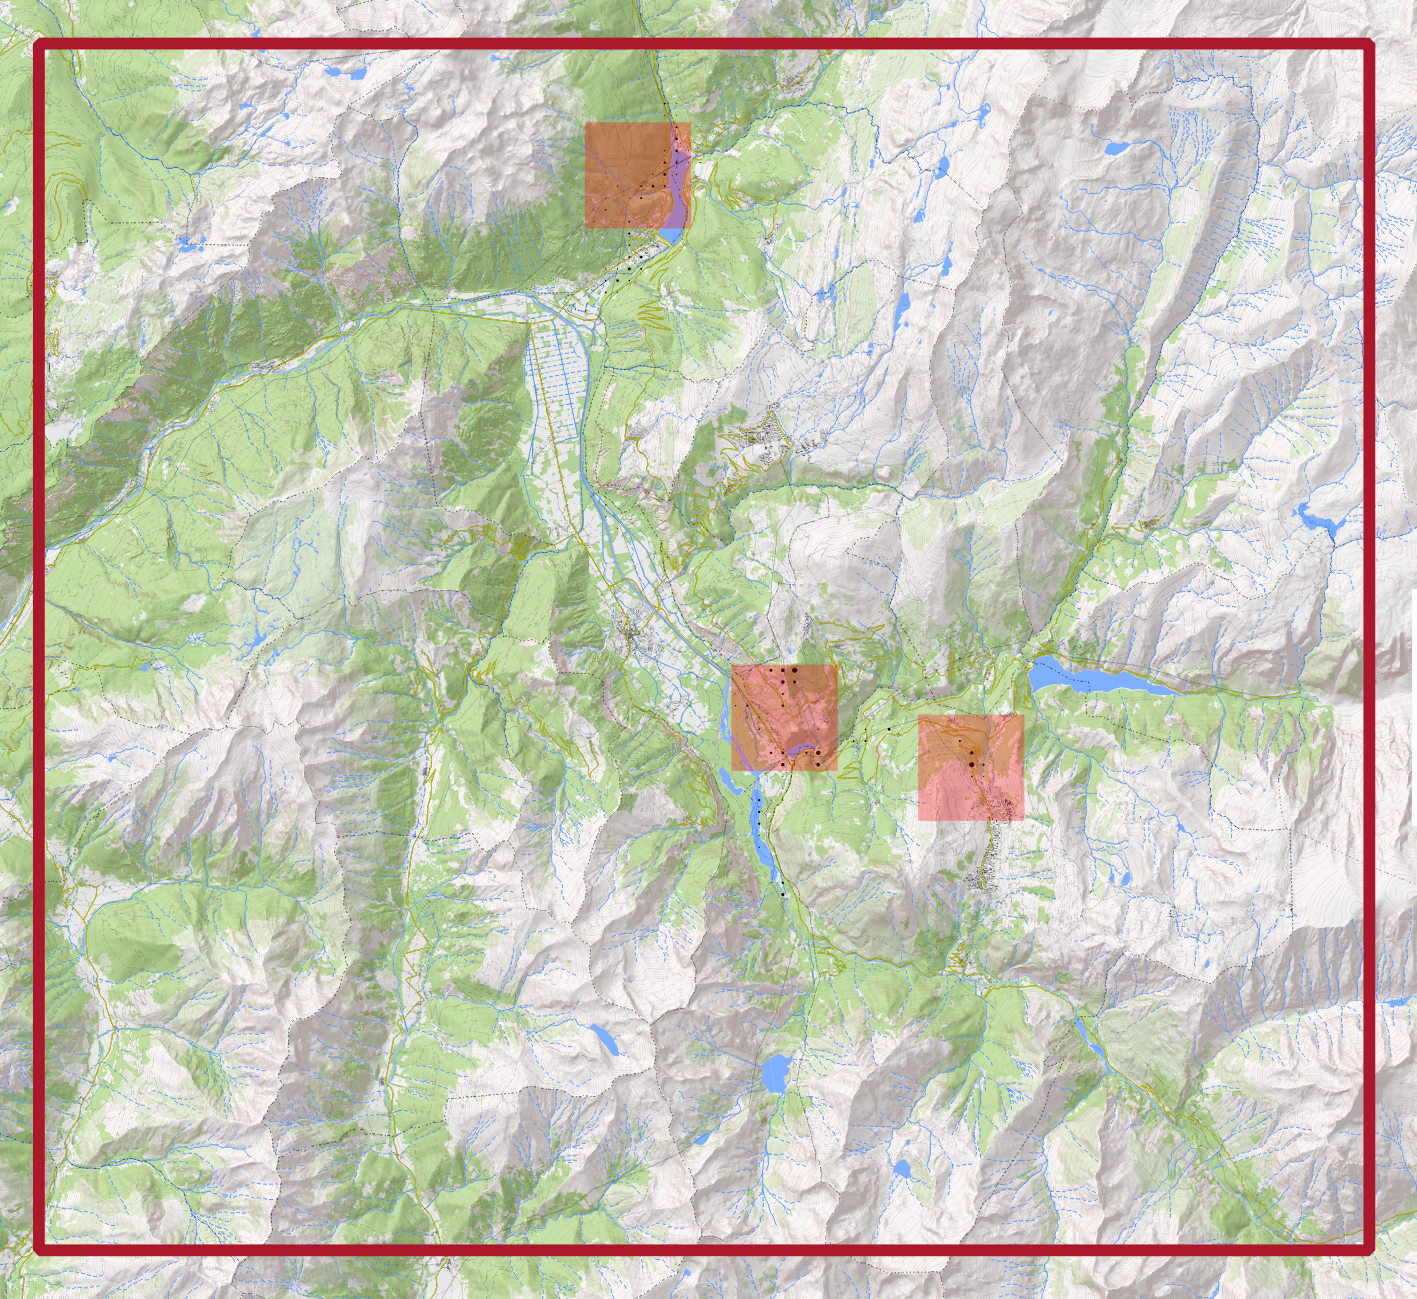
\includegraphics[width=\linewidth]{../figures/ZLP_FilRouge/ZLP.png}};
    \begin{scope}
      \node (P2) at ([yshift=-.5cm]img.south east) {};
      \node (P1) at ([yshift=-.5cm]img.south west) {};
      % 
      \node (rect) [anchor=north west, minimum width=1cm,minimum
      height=.25cm] at ([yshift=-.25cm]P1) {}; \path[draw=RdBu-9-1, line
      width=1mm](rect.west) --([xshift=-1ex]rect.south) -- ([xshift=1ex]rect.north)
      -- (rect.east);
      % 
      \node[anchor=west, font=\tiny\vphantom{Ag}, text width = 4cm] at
      ([xshift=1ex]rect.east) {Limite de la \ac{zir}};
      % 
      \node[anchor=west, font=\footnotesize\vphantom{Ag}] at
      (P1 |- 0cm,-1.7cm) {Degré d'appartenance :};
      % 
      \begin{scope}
        \foreach \x [evaluate=\xshift using 1+\x/10, evaluate=\rad using (\x * .0004) + .01] in {0,...,100}
        {
          \draw[fill=black,draw=none, below] ([xshift=\xshift cm, yshift=-2cm]P1) circle [radius=\rad cm];
        }
        % 
        \path(1,-2.5) --++ (10,0)
        node[et,pos=0] {0}
        node[et,pos=.5] {0,5}
        node[et,pos=1] {1};
      \end{scope}
      % Légende détaillée
      \path (P1) -- (P2) node[pos=.5, yshift=-2.5cm] {\tiny Pour la légende détaillée du fond topographique voir \autoref{anx:topo_leg}. Sources: BD TOPO 2018, BD ALTI 2018.}; 
    \end{scope}
    \begin{scope}[x=(img.south east),y=(img.north west)]
      \node[draw,minimum height=1.6cm,minimum width=1.00cm] (B1) at (0.2,0.60) {};
      \node[draw,minimum height=0.8cm,minimum width=0.50cm] (B2) at (0.7,0.25) {};
      \node[draw,minimum height=0.4cm,minimum width=0.25cm] (B3) at (0.9,0.10) {};
    \end{scope}
  \end{tikzpicture}
}

\subfloat[]{%
  \begin{tikzpicture}[remember picture]
    \tikzset{et/.style={above,font=\footnotesize\vphantom{Ag}}}
    \node (img1)
    {\includegraphics{../figures/ZLP_FilRouge/ZLP_2.png}};
    \draw[-] ([yshift=-.5cm]img1.south east) --++ (-1,0) node[et,pos=.5] {\SI{500}{\meter}};
    \draw (img1.south west) rectangle (img1.north east);
  \end{tikzpicture}
}\hfill
\subfloat[]{%
  \begin{tikzpicture}[remember picture]
    \tikzset{et/.style={above,font=\footnotesize\vphantom{Ag}}}
    \node (img2)
    {\includegraphics{../figures/ZLP_FilRouge/ZLP_3.png}};
    \draw[-] ([yshift=-.5cm]img2.south east) --++ (-1,0) node[et,pos=.5] {\SI{500}{\meter}};
    \draw (img2.south west) rectangle (img2.north east);
  \end{tikzpicture}
}\hfill
\subfloat[]{%
  \begin{tikzpicture}[remember picture]
    \tikzset{et/.style={above,font=\footnotesize\vphantom{Ag}}}
    \node (img3)
    {\includegraphics{../figures/ZLP_FilRouge/ZLP_4.png}};
    \draw[-] ([yshift=-.5cm]img3.south east) --++ (-1,0) node[et,pos=.5] {\SI{500}{\meter}};
    \draw (img3.south west) rectangle (img3.north east);
  \end{tikzpicture}
}
\begin{tikzpicture}[overlay, remember picture]
  \tikzset{et/.style={above,font=\footnotesize\vphantom{Ag}}}
  \draw (B1) -- (img1);
  \draw (B2) -- (img2);
  \draw (B3) -- (img3);
\end{tikzpicture}
  \caption{\ac{zlp} de l'alerte \emph{fil rouge}}
  \label{fig:zlp_fil_rouge}
\end{figure}

\subsection{Critique de la modélisation}
\label{subsec:9-4-3}

La zone de localisation probable obtenue à la suite de la
spatialisation de l'alerte \emph{fil rouge.}


Pb de représentation des géométries

Pour la modélisation du second indice de localisation nous avons
employé la relation de localisaiton
\onto[orl]{A\-Temps\-De\-Marche\-De}, employant le modèle de
\textcite{Tobler1993} par le biais de la métrique
\onto[orla]{Distance\-Temps}. Cependant lors du calcul de la métrique
nous n'avons pas fait varier la valeur du coefficient \(g\) de
\textcite{Tobler1993}, permettant de pénaliser la vitesse de
déplacement si celui-ci est effectué hors sentier. La métrique
représentée sur la \autoref{} est donc sensiblement plus optimiste que
celle qui aurait été obtenue à l'aide d'une implémentation complète du
modèle de \textcite{Tobler1993}.
%
Il est cependant difficile

Pour l'indice \ref{ind:fr4} nous avons pris le parti de limiter les
objets de références

Enfin, le dernier indice de localisation (\ref{ind:fr7}) ne propose
qu'une approximation grossière de l'information contenue dans la
description.
%
Nous pouvons supposer qu'une modélisation plus fine, fondée sur une
relation de localisation adaptée, aurait permis la suppression des
deux clusters de faible degré d'appartenance situés au Nord de
Bourg-d'Oisans.


On peut également critiquer les choix qui ont étés faits pour le
dernier indice de localisaiton

Dans le cas présent, la connaissance de la station de ski visée
(\ref{ind:fr1}), du chemin emprunté (\ref{ind:fr3}) ou même du lac vu
(\ref{ind:fr4}) aurait permis de réduire sensiblement l'étendue de la
\ac{zlp}.

De nombreuses voies sont donc empruntables pour améliorer la
modélisation de cette alerte.


%%% Local Variables:
%%% mode: latex
%%% TeX-master: "../../../../main"
%%% End:
